\documentclass[10pt]{article}\usepackage[]{graphicx}\usepackage[]{color}
%% maxwidth is the original width if it is less than linewidth
%% otherwise use linewidth (to make sure the graphics do not exceed the margin)
\makeatletter
\def\maxwidth{ %
  \ifdim\Gin@nat@width>\linewidth
    \linewidth
  \else
    \Gin@nat@width
  \fi
}
\makeatother

\definecolor{fgcolor}{rgb}{0.345, 0.345, 0.345}
\newcommand{\hlnum}[1]{\textcolor[rgb]{0.686,0.059,0.569}{#1}}%
\newcommand{\hlstr}[1]{\textcolor[rgb]{0.192,0.494,0.8}{#1}}%
\newcommand{\hlcom}[1]{\textcolor[rgb]{0.678,0.584,0.686}{\textit{#1}}}%
\newcommand{\hlopt}[1]{\textcolor[rgb]{0,0,0}{#1}}%
\newcommand{\hlstd}[1]{\textcolor[rgb]{0.345,0.345,0.345}{#1}}%
\newcommand{\hlkwa}[1]{\textcolor[rgb]{0.161,0.373,0.58}{\textbf{#1}}}%
\newcommand{\hlkwb}[1]{\textcolor[rgb]{0.69,0.353,0.396}{#1}}%
\newcommand{\hlkwc}[1]{\textcolor[rgb]{0.333,0.667,0.333}{#1}}%
\newcommand{\hlkwd}[1]{\textcolor[rgb]{0.737,0.353,0.396}{\textbf{#1}}}%
\let\hlipl\hlkwb

\usepackage{framed}
\makeatletter
\newenvironment{kframe}{%
 \def\at@end@of@kframe{}%
 \ifinner\ifhmode%
  \def\at@end@of@kframe{\end{minipage}}%
  \begin{minipage}{\columnwidth}%
 \fi\fi%
 \def\FrameCommand##1{\hskip\@totalleftmargin \hskip-\fboxsep
 \colorbox{shadecolor}{##1}\hskip-\fboxsep
     % There is no \\@totalrightmargin, so:
     \hskip-\linewidth \hskip-\@totalleftmargin \hskip\columnwidth}%
 \MakeFramed {\advance\hsize-\width
   \@totalleftmargin\z@ \linewidth\hsize
   \@setminipage}}%
 {\par\unskip\endMakeFramed%
 \at@end@of@kframe}
\makeatother

\definecolor{shadecolor}{rgb}{.97, .97, .97}
\definecolor{messagecolor}{rgb}{0, 0, 0}
\definecolor{warningcolor}{rgb}{1, 0, 1}
\definecolor{errorcolor}{rgb}{1, 0, 0}
\newenvironment{knitrout}{}{} % an empty environment to be redefined in TeX

\usepackage{alltt}

\usepackage{amsmath,amssymb,amsthm}
\usepackage{fancyhdr,url,hyperref}
\usepackage{graphicx,xspace}
\usepackage{subfigure}
\usepackage{tikz}
\usetikzlibrary{arrows,decorations.pathmorphing,backgrounds,positioning,fit,through}

\oddsidemargin 0in  %0.5in
\topmargin     0in
\leftmargin    0in
\rightmargin   0in
\textheight    9in
\textwidth     6in %6in
%\headheight    0in
%\headsep       0in
%\footskip      0.5in

\newtheorem{thm}{Theorem}
\newtheorem{cor}[thm]{Corollary}
\newtheorem{obs}{Observation}
\newtheorem{lemma}{Lemma}
\newtheorem{claim}{Claim}
\newtheorem{definition}{Definition}
\newtheorem{question}{Question}
\newtheorem{answer}{Answer}
\newtheorem{problem}{Problem}
\newtheorem{solution}{Solution}
\newtheorem{conjecture}{Conjecture}

\pagestyle{fancy}

\lhead{\textsc{Prof. McNamara}}
\chead{\textsc{SDS/MTH 220: Lecture notes}}
\lfoot{}
\cfoot{}
%\cfoot{\thepage}
\rfoot{}
\renewcommand{\headrulewidth}{0.2pt}
\renewcommand{\footrulewidth}{0.0pt}

\newcommand{\ans}{\vspace{0.25in}}
\newcommand{\R}{{\sf R}\xspace}
\newcommand{\cmd}[1]{\texttt{#1}}
\newcommand{\Ex}{\mathbb{E}}

\rhead{\textsc{November 8, 2017}}
\IfFileExists{upquote.sty}{\usepackage{upquote}}{}
\begin{document}

\paragraph{Agenda}
\begin{enumerate}
  \itemsep0em
  \item Goodness of fit
\end{enumerate}

\paragraph{Goodness of Fit}

Previously, we considered inference for a single proportion. That proportion was the fraction of the outcomes of a binary response variable that had a certain value. For example, respondents could either say that they preferred Coke, or that they preferred Pepsi. But what if the variable can have more than two outcomes? Can we still test the hypothesis that the sample was drawn from a known population? 

The \href{https://www.census.gov/prod/2003pubs/c2kbr-30.pdf}{US Census Bureau} reports that in 2000, among the population 15 years and older:
\begin{itemize}
  \itemsep0in
  \item 54.3\% are married
  \item 27.1\% have never been married
  \item 9.7\% are divorced
  \item 6.6\% are widowed
  \item 2.2\% are separated
\end{itemize}

We can encode these percentages as a vector in \R:

\begin{knitrout}\footnotesize
\definecolor{shadecolor}{rgb}{0.969, 0.969, 0.969}\color{fgcolor}\begin{kframe}
\begin{alltt}
\hlstd{us} \hlkwb{<-} \hlkwd{c}\hlstd{(}\hlstr{"Divorced"} \hlstd{=} \hlnum{0.097}\hlstd{,} \hlstr{"Married"} \hlstd{=} \hlnum{0.543}\hlstd{,} \hlstr{"Never married/single"} \hlstd{=} \hlnum{0.271}\hlstd{,}  \hlstr{"Separated"} \hlstd{=} \hlnum{0.022}\hlstd{,} \hlstr{"Widowed"} \hlstd{=} \hlnum{0.066}\hlstd{)}
\hlcom{# normalize to make sure proportions sum to 1}
\hlstd{us} \hlkwb{<-} \hlstd{us} \hlopt{/} \hlkwd{sum}\hlstd{(us)}
\hlstd{us}
\end{alltt}
\begin{verbatim}
##             Divorced              Married Never married/single 
##           0.09709710           0.54354354           0.27127127 
##            Separated              Widowed 
##           0.02202202           0.06606607
\end{verbatim}
\end{kframe}
\end{knitrout}

The \cmd{openintro} package contains a sample of 500 Americans collected in the 2000 Census. In this sample, the percentages are different: 

\begin{knitrout}\footnotesize
\definecolor{shadecolor}{rgb}{0.969, 0.969, 0.969}\color{fgcolor}\begin{kframe}
\begin{alltt}
\hlkwd{library}\hlstd{(openintro)}
\hlkwd{library}\hlstd{(mosaic)}
\hlstd{marital_summary} \hlkwb{<-} \hlstd{census} \hlopt
  \hlkwd{mutate}\hlstd{(}\hlkwc{maritalStatus} \hlstd{=}
           \hlstd{forcats}\hlopt{::}\hlkwd{fct_recode}\hlstd{(maritalStatus,} \hlkwc{Married} \hlstd{=} \hlstr{"Married/spouse absent"}\hlstd{,}
                               \hlkwc{Married} \hlstd{=} \hlstr{"Married/spouse present"}\hlstd{))} \hlopt
  \hlkwd{group_by}\hlstd{(maritalStatus)} \hlopt
  \hlkwd{summarize}\hlstd{(}\hlkwc{status_obs} \hlstd{=} \hlkwd{n}\hlstd{())} \hlopt
  \hlkwd{mutate}\hlstd{(}\hlkwc{marital_status_pct} \hlstd{= status_obs} \hlopt{/} \hlkwd{nrow}\hlstd{(census),} \hlkwc{marital_status_us} \hlstd{= us)}
\hlstd{marital_summary}\hlopt{$}\hlstd{marital_status_pct}
\end{alltt}
\begin{verbatim}
## [1] 0.076 0.412 0.444 0.006 0.062
\end{verbatim}
\end{kframe}
\end{knitrout}

Is it reasonable to conclude that the sample from 2000 reflects the overall US population? 

In the previous case, the test statistic was the observed sample proportion $\hat{p}$. In this case, we have more than two outcomes, so there is nothing quite analogous to $\hat{p}$. The test statistic that we will use will be labelled $X^2$, and its formula is:

$$
  X^2 = \sum_{i=1}^k Z_i^2 = \sum_{i=1}^k \left( \frac{observed_i - expected_i}{\sqrt{expected_i}} \right)^2 = \sum_{i=1}^k \frac{(observed_i - expected_i)^2}{expected_i} \,,
$$
where $k$ is the number of different outcomes (which in this case is 5). As always, our goal is to put $X^2$ in context by determining where it lies in the null distribution. First, let's compute the test statistic:

\begin{knitrout}\footnotesize
\definecolor{shadecolor}{rgb}{0.969, 0.969, 0.969}\color{fgcolor}\begin{kframe}
\begin{alltt}
\hlstd{n} \hlkwb{<-} \hlkwd{nrow}\hlstd{(census)}
\hlstd{k} \hlkwb{<-} \hlkwd{nrow}\hlstd{(marital_summary)}
\hlstd{marital_summary} \hlkwb{<-} \hlstd{marital_summary} \hlopt
  \hlkwd{mutate}\hlstd{(}\hlkwc{status_exp} \hlstd{= marital_status_us} \hlopt{*} \hlstd{n)}
\hlstd{X2_hat} \hlkwb{<-} \hlstd{marital_summary} \hlopt
  \hlkwd{summarize}\hlstd{(}\hlkwc{X2} \hlstd{=} \hlkwd{sum}\hlstd{(((status_obs} \hlopt{-} \hlstd{status_exp)}\hlopt{^}\hlnum{2}\hlstd{)} \hlopt{/} \hlstd{status_exp))} \hlopt \hlkwd{unlist}\hlstd{()}
\end{alltt}
\end{kframe}
\end{knitrout}




\begin{enumerate}
  \item Write out the full calculation for $X^2$ using a table
  \vspace{2in}
\end{enumerate}

We want to test the null hypothesis that our sample came from the population, whose marital status breakdown is known. Since this implies that the observed counts will match the expected counts exactly, this would result in a test statistic of $\hat{X^2} = 0$. Our observed value of $\hat{X^2}$ is very different from 0, but in order to understand \emph{how} different, we need to know what the null distribution of $\hat{X^2}$ is. In this case, it is \emph{not} normal! 

Just as before, there are at least three different ways to construct the sampling distribution of $\hat{X^2}$:

\begin{enumerate}
  \item Simulation: The procedure is the same it has been: sample from the hypothesized distribution and compute the test statistic many thousands of times. 

\begin{knitrout}\footnotesize
\definecolor{shadecolor}{rgb}{0.969, 0.969, 0.969}\color{fgcolor}\begin{kframe}
\begin{alltt}
\hlstd{sim} \hlkwb{<-} \hlkwd{do}\hlstd{(}\hlnum{1000}\hlstd{)} \hlopt{*}
  \hlstd{marital_summary} \hlopt
  \hlkwd{sample_n}\hlstd{(}\hlkwc{size} \hlstd{= n,} \hlkwc{replace} \hlstd{=} \hlnum{TRUE}\hlstd{,} \hlkwc{weight} \hlstd{= marital_status_us)} \hlopt
  \hlkwd{group_by}\hlstd{(maritalStatus)} \hlopt
  \hlkwd{summarize}\hlstd{(}\hlkwc{status_obs} \hlstd{=} \hlkwd{n}\hlstd{(),} \hlkwc{status_exp} \hlstd{=} \hlkwd{first}\hlstd{(status_exp))} \hlopt
  \hlkwd{mutate}\hlstd{(}\hlkwc{X2_i} \hlstd{= (status_obs} \hlopt{-} \hlstd{status_exp)}\hlopt{^}\hlnum{2} \hlopt{/} \hlstd{status_exp)} \hlopt
  \hlkwd{summarize}\hlstd{(}\hlkwc{X2} \hlstd{=} \hlkwd{sum}\hlstd{(X2_i))}
\hlkwd{qplot}\hlstd{(}\hlkwc{data} \hlstd{= sim,} \hlkwc{x} \hlstd{= X2)}
\end{alltt}
\end{kframe}
\end{knitrout}

  The p-value can be obtained using the \cmd{pdata} function, since the sampling distribution comes from simulated data in our workspace. Note also that since the distribution is non-negative, our test is one-sided. 

\begin{knitrout}
\definecolor{shadecolor}{rgb}{0.969, 0.969, 0.969}\color{fgcolor}\begin{kframe}
\begin{alltt}
\hlkwd{pdata}\hlstd{(}\hlopt{~}\hlstd{X2, X2_hat,} \hlkwc{data} \hlstd{= sim,} \hlkwc{lower.tail} \hlstd{=} \hlnum{FALSE}\hlstd{)}
\end{alltt}
\begin{verbatim}
## X2 
##  0
\end{verbatim}
\end{kframe}
\end{knitrout}
  
  
  \item Probability Theory: Last time, we worked with a \emph{binary} variable, and that led to a \emph{binomial} distribution. This time, we have a categorical variable that can take on more than two values, and that leads to a \emph{multinomial} distribution. For the purposes of this class, you do not need to know what a multinomial distribution is, but it is the multivariate extension of the binomial distribution (i.e. the binomial distribution is the special case of the multinomial distribution when the number of outcomes is 2).
  
  We will not discuss this approach any further, but based on what you saw last time, hopefully you can believe us that: a) it exists; b) it requires some non-trivial probability theory; and c) it is computationally burdensome. 
  
  \item Chi-Squared Test: Since the multinomial distribution is very cumbersome to work with, statisticians have constructed a parametric approximation to the sampling distribution of $\hat{X^2}$. It follows from probability theory that as long as the expected count of each outcome is at least 5, the test statistic follows a distribution that is closely approximated by a $\chi^2$-distribution on $k-1$ degrees of freedom. 
  
\begin{knitrout}
\definecolor{shadecolor}{rgb}{0.969, 0.969, 0.969}\color{fgcolor}\begin{kframe}
\begin{alltt}
\hlkwd{plotDist}\hlstd{(}\hlstr{"chisq"}\hlstd{,} \hlkwc{params} \hlstd{=} \hlkwd{list}\hlstd{(}\hlkwc{df} \hlstd{= k}\hlopt{-}\hlnum{1}\hlstd{),} \hlkwc{lwd} \hlstd{=} \hlnum{3}\hlstd{)}
\end{alltt}
\end{kframe}
\end{knitrout}

The p-value can be obtained using the \cmd{pchisq} function, since the sampling distribution follows a $\chi^2$-distribution.

\begin{knitrout}
\definecolor{shadecolor}{rgb}{0.969, 0.969, 0.969}\color{fgcolor}\begin{kframe}
\begin{alltt}
\hlkwd{pchisq}\hlstd{(X2_hat,} \hlkwc{df} \hlstd{= k}\hlopt{-}\hlnum{1}\hlstd{,} \hlkwc{lower.tail} \hlstd{=} \hlnum{FALSE}\hlstd{)}
\end{alltt}
\begin{verbatim}
##          X2 
## 2.63096e-16
\end{verbatim}
\end{kframe}
\end{knitrout}

  Notice that the p-value is a one-tailed area in this case, since the distribution is non-negative. 

  There is also a built-in function in \R that will perform a $\chi^2$-test. 
  
\begin{knitrout}\footnotesize
\definecolor{shadecolor}{rgb}{0.969, 0.969, 0.969}\color{fgcolor}\begin{kframe}
\begin{alltt}
\hlkwd{with}\hlstd{(marital_summary,} \hlkwd{chisq.test}\hlstd{(status_obs,} \hlkwc{p} \hlstd{= marital_status_us))}
\end{alltt}
\begin{verbatim}
## 
## 	Chi-squared test for given probabilities
## 
## data:  status_obs
## X-squared = 79.154, df = 4, p-value = 2.631e-16
\end{verbatim}
\end{kframe}
\end{knitrout}

\end{enumerate}


\paragraph{What Can Go Wrong?}

Once again, the condition that the expected count for each category is at least 5 is important, because if that condition is not met, the $\chi^2$-distribution may not be a sufficiently good approximation. Note that the deviation in each count is approximately normal, so the approximation can fail for any of the outcomes. 

\begin{knitrout}\footnotesize
\definecolor{shadecolor}{rgb}{0.969, 0.969, 0.969}\color{fgcolor}\begin{kframe}
\begin{alltt}
\hlstd{n} \hlkwb{<-} \hlnum{35}
\hlstd{sim} \hlkwb{<-} \hlkwd{do}\hlstd{(}\hlnum{1000}\hlstd{)} \hlopt{*}
  \hlstd{marital_summary} \hlopt
  \hlkwd{mutate}\hlstd{(}\hlkwc{status_exp} \hlstd{= marital_status_us} \hlopt{*} \hlstd{n)} \hlopt
  \hlkwd{sample_n}\hlstd{(}\hlkwc{size} \hlstd{= n,} \hlkwc{replace} \hlstd{=} \hlnum{TRUE}\hlstd{,} \hlkwc{weight} \hlstd{= marital_status_us)} \hlopt
  \hlkwd{group_by}\hlstd{(maritalStatus)} \hlopt
  \hlkwd{summarize}\hlstd{(}\hlkwc{status_obs} \hlstd{=} \hlkwd{n}\hlstd{(),} \hlkwc{status_exp} \hlstd{=} \hlkwd{first}\hlstd{(status_exp))} \hlopt
  \hlkwd{mutate}\hlstd{(}\hlkwc{X2_i} \hlstd{= (status_obs} \hlopt{-} \hlstd{status_exp)}\hlopt{^}\hlnum{2} \hlopt{/} \hlstd{status_exp)} \hlopt
  \hlkwd{summarize}\hlstd{(}\hlkwc{X2} \hlstd{=} \hlkwd{sum}\hlstd{(X2_i))}
\hlkwd{qplot}\hlstd{(}\hlkwc{data} \hlstd{= sim,} \hlkwc{x} \hlstd{= X2,} \hlkwc{geom} \hlstd{=} \hlstr{"density"}\hlstd{)} \hlopt{+}
  \hlkwd{stat_function}\hlstd{(}\hlkwc{fun} \hlstd{= dchisq,} \hlkwc{args} \hlstd{=} \hlkwd{list}\hlstd{(}\hlkwc{df} \hlstd{= k}\hlopt{-}\hlnum{1}\hlstd{),} \hlkwc{color} \hlstd{=} \hlstr{"purple"}\hlstd{)}
\end{alltt}
\end{kframe}
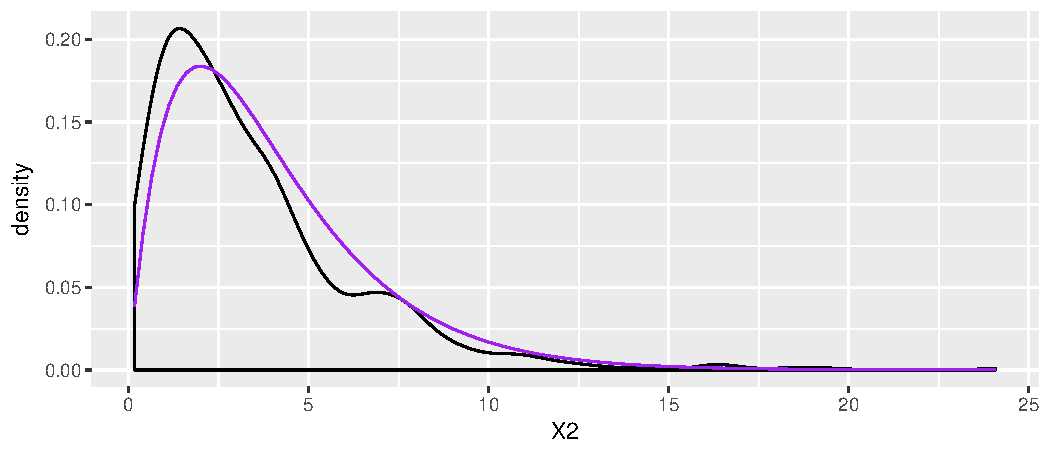
\includegraphics[width=\maxwidth]{figure/unnamed-chunk-10-1} 

\end{knitrout}


\paragraph{In-Class Exercise, OI, 3.40}

\textbf{Evolution vs. creationism} A Gallup Poll released in December 2010 asked 1019 adults living in the Continental U.S. about their belief in the origin of humans. These results, along with results from a more comprehensive poll from 2001 (that we will assume to be exactly accurate), are summarized in the table below: 
\begin{center}
\begin{tabular}{l c c}
  										& \multicolumn{2}{c}{\textit{Year}} \\
\cline{2-3}
\textit{Response}								& 2010	& 2001 \\
\hline
Humans evolved, with God guiding (1)				& 38\% 	& 37\% \\
Humans evolved, but God had no part in process (2) 	& 16\% 	& 12\% \\
God created humans  in present form (3) 				& 40\% 	& 45\% \\
Other / No opinion (4)							& 6\% 	& 6\% \\
\hline
\end{tabular}
\end{center} 

\begin{enumerate}
  \itemsep1.5in
\item Calculate the actual number of respondents in 2010 that fall in each response category.
\item State hypotheses for the following research question: have beliefs on the origin of human life changed since 2001?
\item Calculate the expected number of respondents in each category under the condition that the null hypothesis is true.
\item Conduct a chi-square test and state your conclusion. (Reminder: verify conditions.)
\end{enumerate}

% 
% \newpage
% 
% \paragraph{Solution to Exercise}
% 
% \begin{enumerate}
% \item $O_{(1)} = 1,019 \times  0.38 = 387$ \\
% $O_{(2)} = 1,019 \times  0.16 = 163$ \\
% $O_{(3)} = 1,019 \times  0.40= 408$ \\
% $O_{(4)} = 1,019 \times  0.06 = 61$
% \item The hypotheses are as follows:
% \begin{description}
% \item[] $H_0$: Distribution of the belief in evolutionary origins of humans has not changed from 2001 to 2010.
% \item[] $H_A$: Distribution of the belief in evolutionary origins of humans has changed from 2001 to 2010.
% \end{description}
% 
% \item  $E_{(1)} = 1,019 \times  0.37 = 377$ \\
% $E_{(2)} = 1,019 \times  0.12 = 122$ \\
% $E_{(3)} = 1,019 \times  0.45= 459$ \\
% $E_{(4)} = 1,019 \times  0.06 = 61$
% \item Before calculating the test statistic we should check that the conditions are satisfied. 
% \begin{description}
% \item Independence:  The sample is random, and 1,019 $<$ 10\% of all Americans, therefore respondents' answers are independent of each other.
% \item Sample size: All expected counts are at least 5.
% \item Degrees of freedom: $df = k - 1 = 4 - 1 = 3 > 2$.
% \end{description}
% 
% The chi-squared statistic, the degrees of freedom associated with it, and the p-value can be calculated as follows:
% \begin{align*}
% X^2 &= \sum \frac{(O - E)^2}{E} =  \frac{(387 - 377)^2} {377} + \frac{(163 - 122)^2} {122} + \frac{(408 - 459)^2} {459} + \frac{(61 - 61)^2}{61} = 19.71 \\
% df &= 3 \\
% p-value &< 0.001
% \end{align*}
% 
% Since the p-value $< \alpha$, we reject $H_0$. The data provide strong evidence that the distribution of the belief in evolutionary origins of humans has changed from 2001 to 2010. Since an increase was observed in the response ``Humans evolved, but God had no part in process" there is support for the comment.
% \end{enumerate}

\end{document}
